\chapter{Interaction between Languages}

After providing scheme, lua support into the browser, we needed a way for this language to interact with each other. 

Every language is different, and achieving even slight levels of language interoperability is pretty difficult because the wide variation in programming language features, and implementations. after going through all the challenges and possible solution, For this project, we decided to take approach which will be similar to Nashorn \cite{Juneau2017}, code from other languages can be called by using the helper evaluate function provided by that language.

All languages will provide evaluate function, which will evaluate code native to that language and will return the results.

We will see the interaction between different languages with examples, in following sections.

\section{Scheme to JS Interaction}

Our implementation of scheme provides, evaluate function called "js-eval", which takes argument of java script code in string, and it executes that java script code from scheme environment, as shown in example below,

\begin{lstlisting}[frame=single]
<!DOCTYPE html>
<html>
<head>
<title>Calling Java Script from Scheme example</title>
</head>

<body>
<input type="button" id="call" 
value="Click to call Java Script from Scheme" />

</body>
<script type="text/scheme">
(
  (add-handler! "#call" "click" (lambda(ev)
    (js-eval "var sayHello = function (tmp) {
                                   return 'Hello ' + tmp
                                 };"
    )
    (js-eval "alert('Java Script Alert from Scheme - ' 
     + sayHello('Swapnil'))")))
  )
 )
</script>
\end{lstlisting}

The above code, adds a click handler to input button with id "call", after clicking a button it executes a js-eval function of scheme, which creates javascript function called sayHello, and then next line executes that Java Script function by passing arguments to it.  Output generated by above code is shown in the figure \ref{fig:scheme-js-interaction}.

\begin{figure}[H]
	\begin{center}
		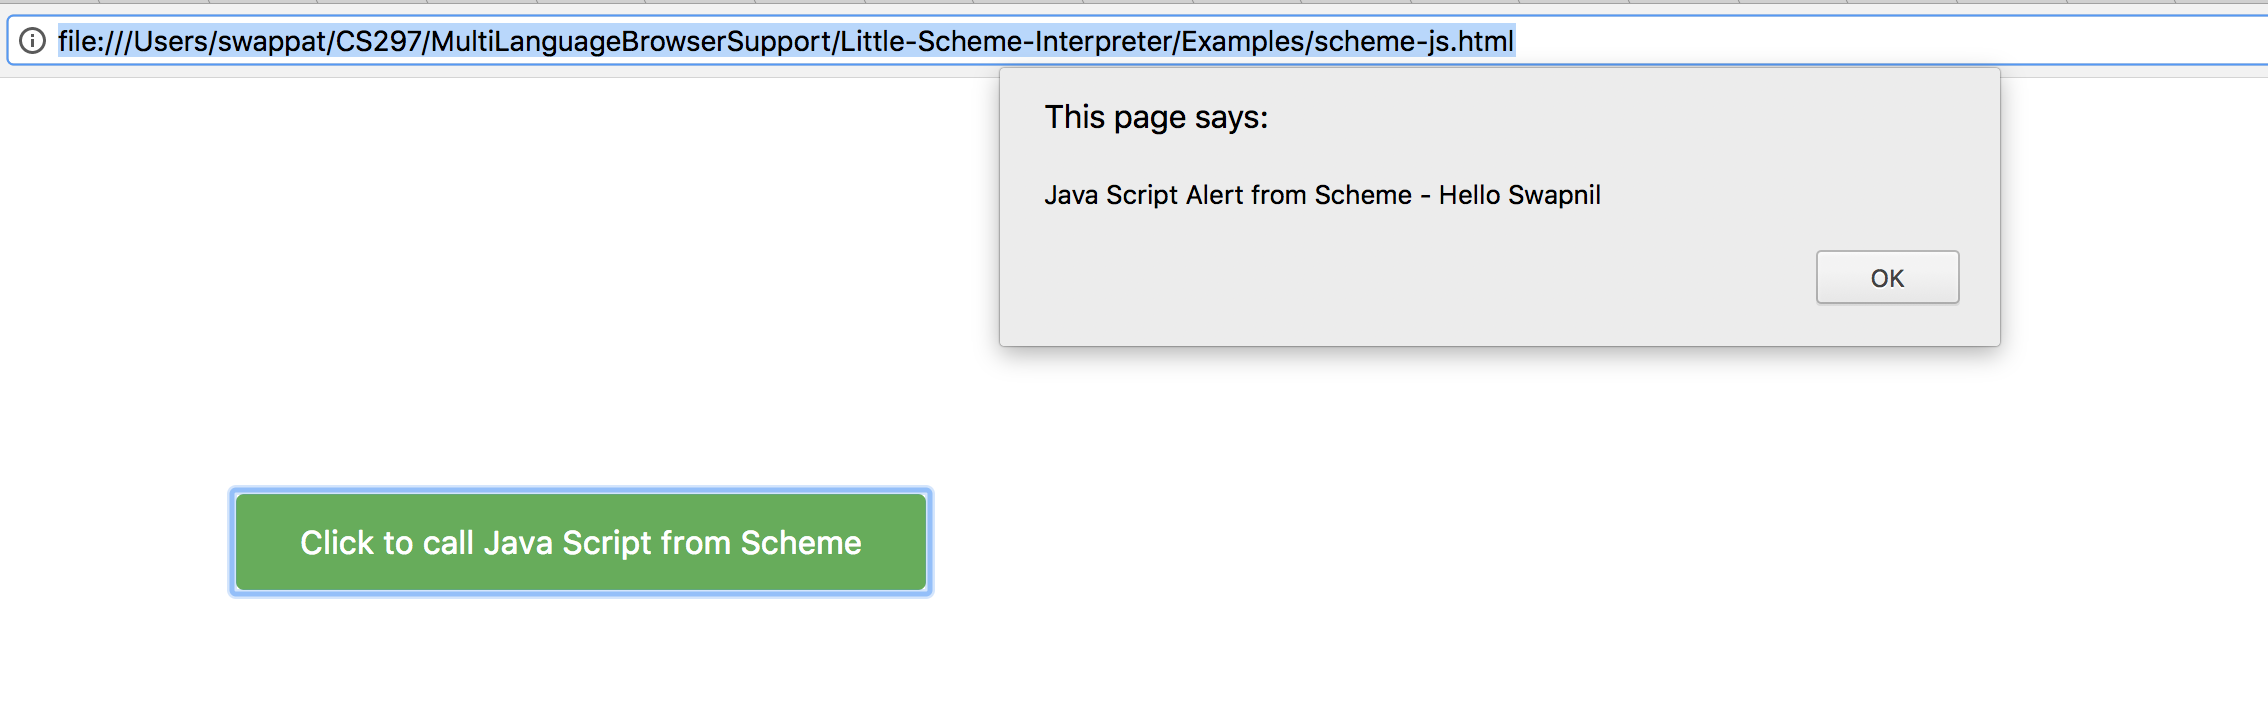
\includegraphics[width=\linewidth]{./images/scheme-js-interaction.png}
	\end{center}
	\caption{Executing Java Script from Scheme: Output}
	\label{fig:scheme-js-interaction}
\end{figure}


\section{JS to Scheme Interaction}

Similar, to calling Java Script code from scheme, we can also execute scheme code from java script. Web page, gets the instance of our scheme interpreter, by calling evaluate method on that instance, java script can execute scheme code, as shown in code below, 

\begin{lstlisting}[frame=single]
<!DOCTYPE html>
<html>
<head>
<meta charset="utf-8" />
<title>Calling Schemet from Java Scriptexample</title>
</head>
<body>
<input type="button" onclick="callScheme()" 
id="call" value="Execute Scheme Code from Java Script">
</body>
<script>
function callScheme()
{
 var sayHello = scheme.evaluate("(lambda (msg)  (alert msg) )");
 sayHello("Calling scheme method from Java Script!!!!!");
}
</script>
</html>
\end{lstlisting}

In the above code, we are evaluating function written in scheme, and calling it from Java Script. "scheme.evaluate" functions executes the scheme code, In this case, we are storing scheme lambda function in variable called sayHello, and calling it with parameters from Java Script, as shown in figure \ref{fig:js-scheme-interaction}

\begin{figure}[H]
	\begin{center}
		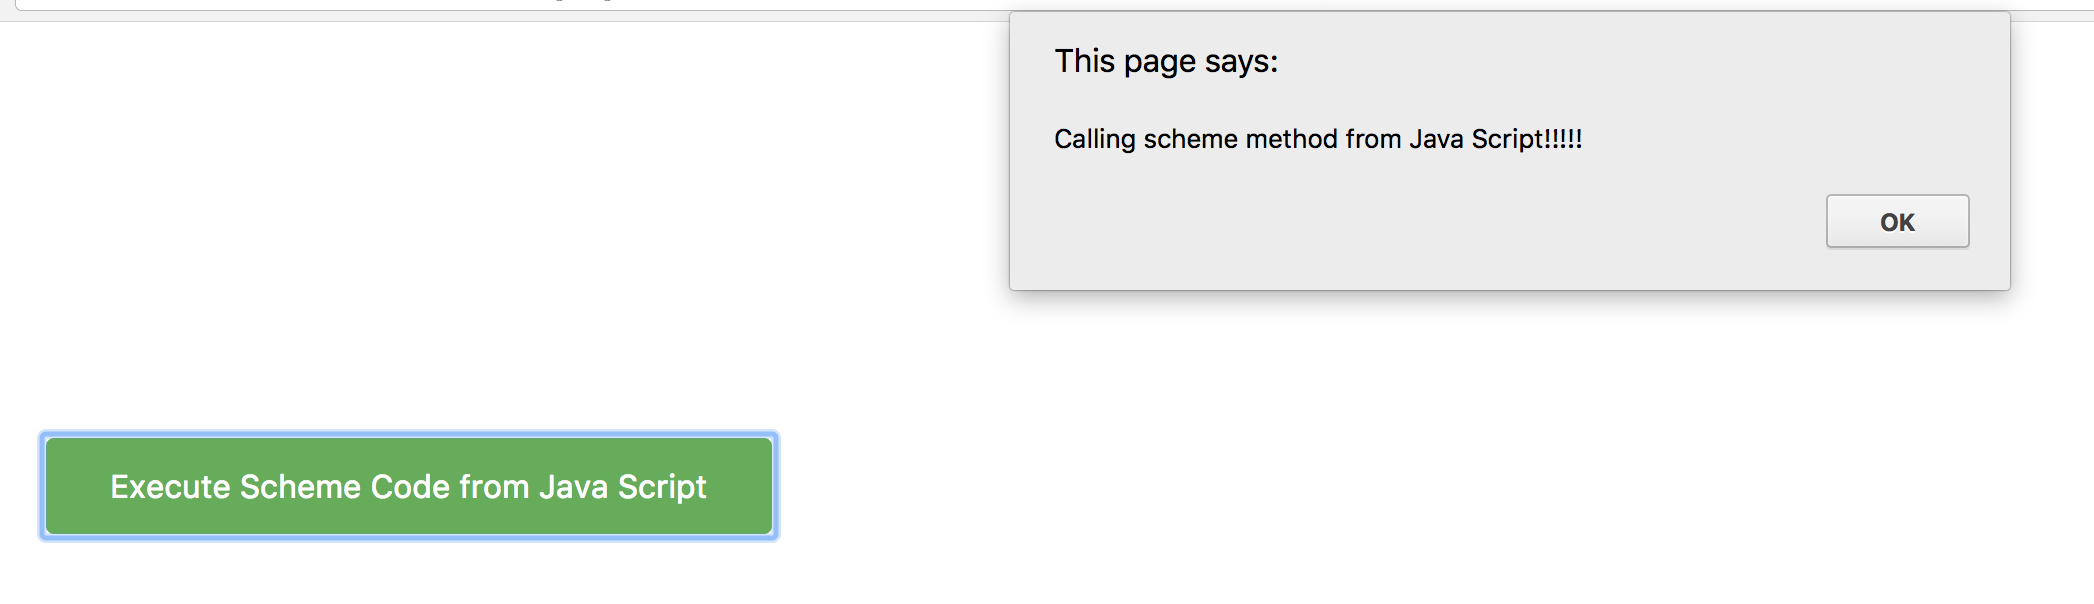
\includegraphics[width=\linewidth]{./images/js-scheme-interaction.png}
	\end{center}
	\caption{Executing Scheme from Java Script: Output}
	\label{fig:js-scheme-interaction}
\end{figure}


\section{Lua to JS Interaction}

Lua interacts with Java Script using eval function on Java Script global object, following code snippet shows, how to write lua code in the Lua script, and highlighted code shows, how to access, Java Script code from Lua script.

\begin{lstlisting}[frame=single, style=base]
<html>
<head>
<script src="lua.vm.js"></script>

<title>Lua VM - Lua to JS interaction</title>
<script type="text/lua">

local window = js.global -- global object in JS is the window

@-- Lua executing Java Script code
window:eval('function sayHello (message)' ..
 '{ alert(message); }' ..
 'sayHello("Hello from Java Script calling from Lua");'
) @

-- Alert from Lua
window:alert("hello from lua!")


-- Accessing DOM APIS from Lua
local document = js.global.document
print("This window has title '" .. document.title .. "'")

-- function
function printWindowSize ()
 local screen = js.global.screen
 print("you haz " .. (screen.width*screen.height) .. " pixels")
end

printWindowSize()
</script>

</head>
<body>
 Executing lua function in browser.
</body>
</html>
\end{lstlisting}

In the code snippet above, highlighted code, Lua environment is creating Java Script function called "sayHello", and it is calling it using eval function on Java Script global object. Output of above code snippet is shown in figures \ref{fig:alert-from-javascript-eval} \ref{fig:alert-from-lua} \ref{fig:printing-document-title}

\begin{figure}[H]
	\begin{center}
		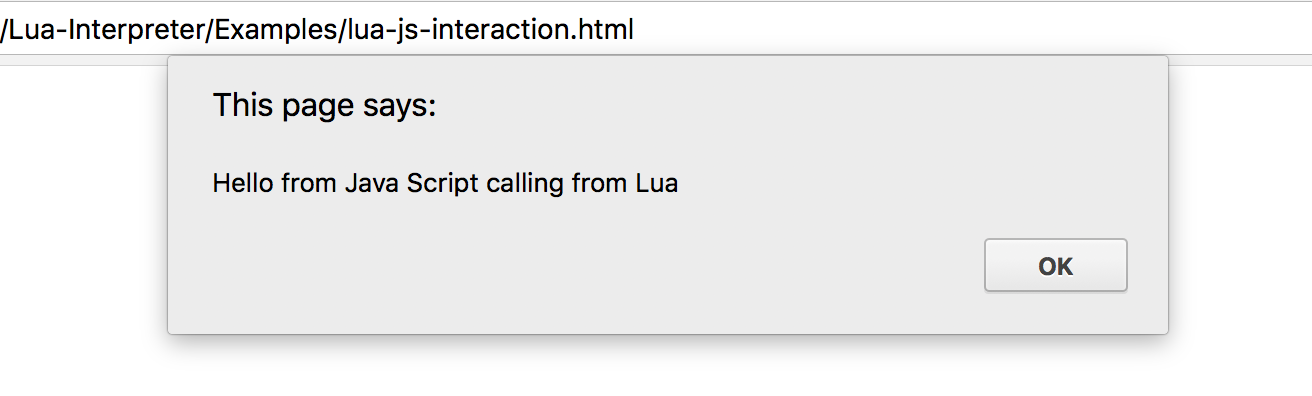
\includegraphics[width=\linewidth]{./images/alert-from-javascript-eval.png}
	\end{center}
	\caption{Executing JS from Lua Script: Output}
	\label{fig:alert-from-javascript-eval}
\end{figure}

\begin{figure}[H]
	\begin{center}
		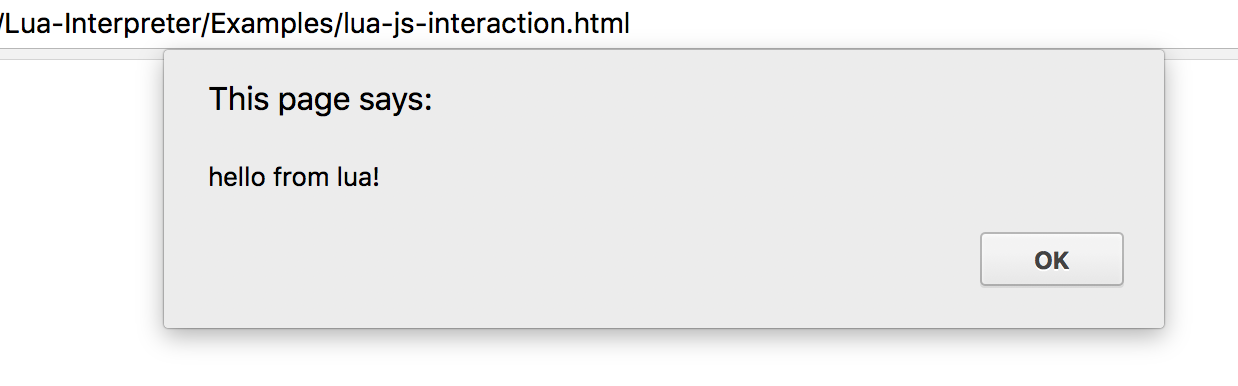
\includegraphics[width=\linewidth]{./images/alert-from-lua.png}
	\end{center}
	\caption{Alert from Lua : Output}
	\label{fig:alert-from-lua}
\end{figure}

\begin{figure}[H]
	\begin{center}
		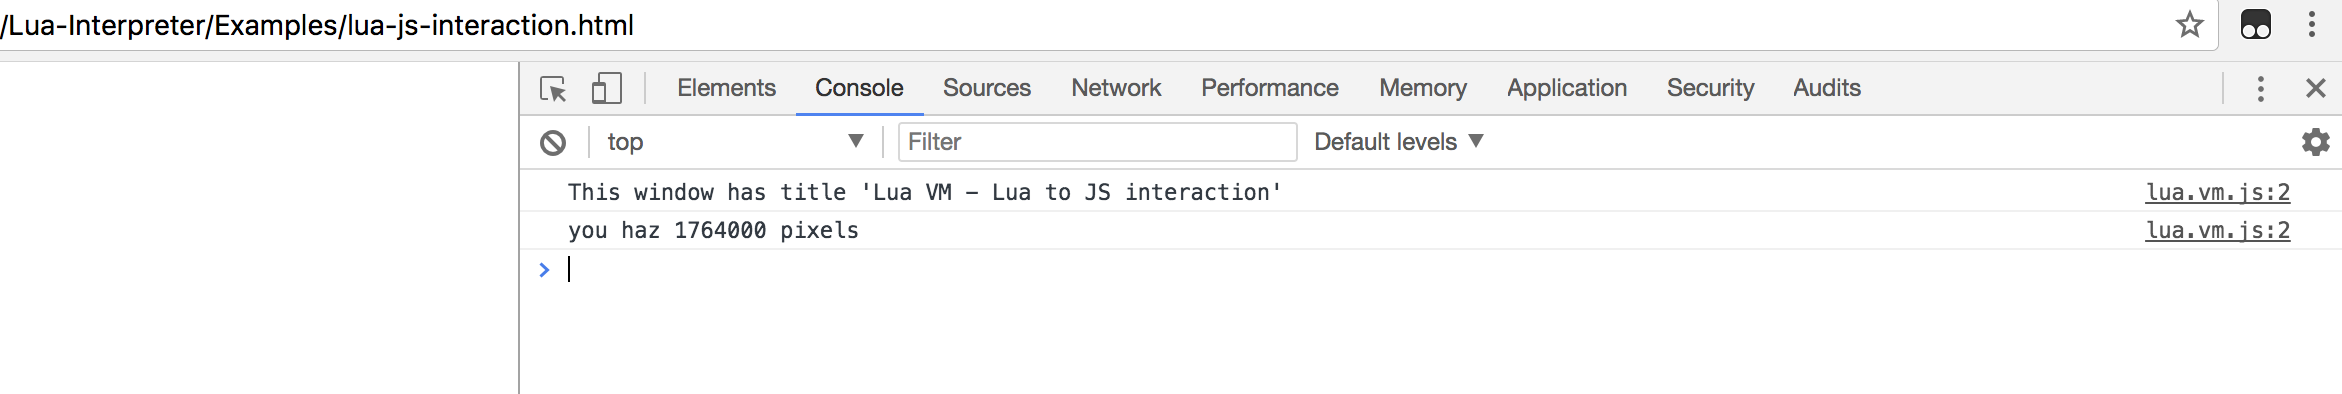
\includegraphics[width=\linewidth]{./images/printing-document-title.png}
	\end{center}
	\caption{Accessing DOM from Lua : Output}
	\label{fig:printing-document-title}
\end{figure}

\section{JS to Lua Interaction}

Java Script interacts with Lua, using the L.execute function provides by Lua VM, It accepts any lua code as a string, and it executes it in Java Script environment by calling the function, as shown in code snippet below, 


\begin{lstlisting}[frame=single, style=base]
<html>
<head>
<script src="lua.vm.js"></script>

<title>Lua VM </title>

<script>
function sayHello(message) {
 console.log(message);
}

@L.execute( // Lua Function Declaration
 "function printName (recipient) " +
 "print('Hello, '..recipient)" +
 "end " +

 // Call to Lua Function
 "printName('CS298 Project') " +

 // Calling Java Script function from Lua 
 "js.global:sayHello('Hello to JS function')" +

 // Alert from Lua " 
 "js.global:alert('Hello from Lua') "
); @

</script>
</head>
<body>
Executing lua function from Java Script environment.
</body>
</html>
\end{lstlisting}

Above code snippet calls lua code from Java Script environment. It creates Lua function called printName which prints the message on the console, this function is called with parameter "CS 298 Project". It also calls Java Script function called "sayHello" from Lua code. and similary, it alert the "Hello from Lua" message using scheme alert function. Output of the above code snippet is shown in the figure \ref{fig:js-to-lua-interaction}

\begin{figure}[H]
	\begin{center}
		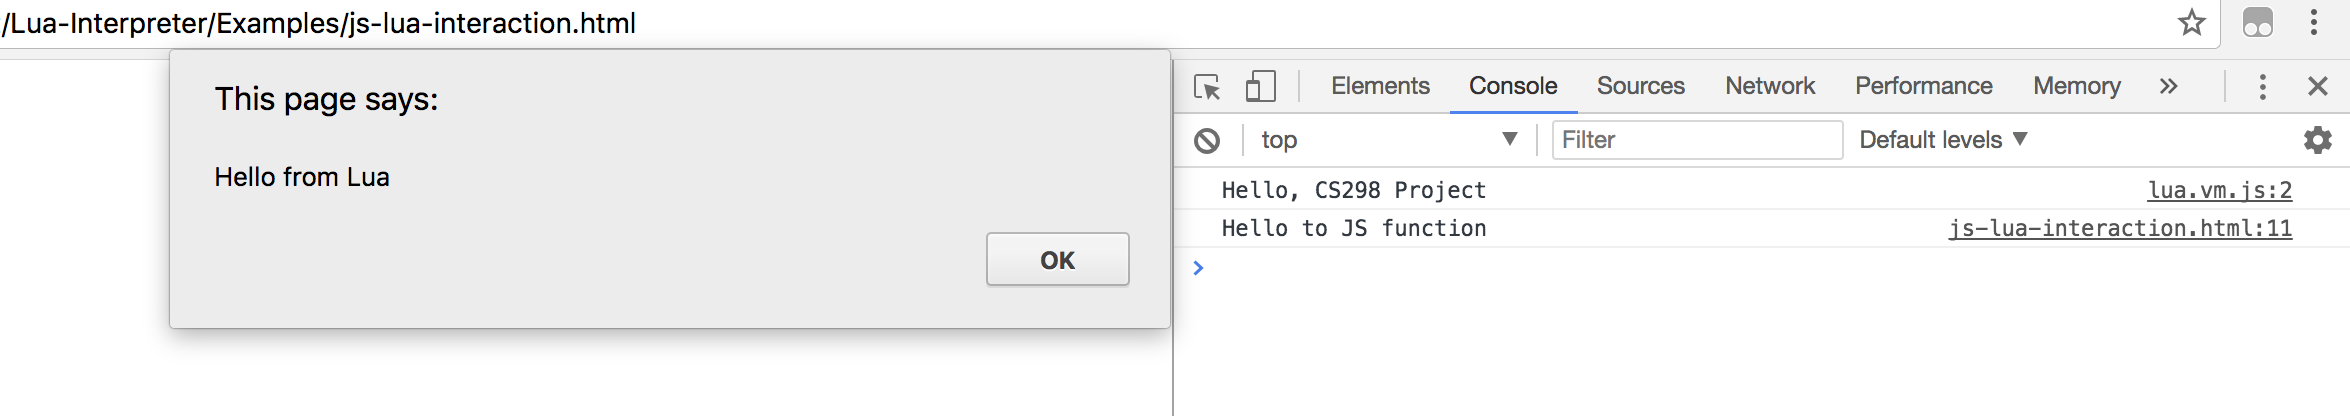
\includegraphics[width=\linewidth]{./images/js-to-lua-interaction.png}
	\end{center}
	\caption{Accessing Lua from JS : Output}
	\label{fig:js-to-lua-interaction}
\end{figure}


